\documentclass[11pt,a4paper]{article}
\usepackage[margin=23mm]{geometry}
\usepackage[T1]{fontenc}
\usepackage{lmodern,amsmath,amssymb,amsthm,booktabs,array,enumitem,xcolor}
\usepackage[colorlinks=true,linkcolor=blue!50!black,urlcolor=blue!50!black]{hyperref}
\usepackage{xurl}
\usepackage{tikz}
\usetikzlibrary{arrows.meta,positioning}
\setlength{\parindent}{0pt}
\setlength{\parskip}{6pt}
\setlength{\emergencystretch}{3em}
\setlist{nosep,leftmargin=*}
\newcommand{\OPT}{\operatorname{OPT}}
\newcommand{\cost}{\operatorname{cost}}
\newcommand{\clog}{\operatorname{clog}_2}
\newcommand{\lean}[1]{{\small\expandafter\nolinkurl\expandafter{\detokenize{#1}}}}
\newcommand{\source}[1]{\par\smallskip{\small\textbf{Lean map.} #1}\par}
\newcommand{\checked}{\textbf{Checked ingredients.}}
\newcommand{\pending}{\textbf{Remaining assembly.}}
\newcommand{\nextpage}{\clearpage}
\newtheorem{definition}{Definition}[section]
\newtheorem{claim}[definition]{Claim}
\begin{document}
\begin{center}
{\Large\bfseries Cha-Cha: from the paper to Lean}\\[4pt]
{\large A proof guide and a route to classical MultiSplay}\\[3pt]
Working document, 1 November 2026
\end{center}

\section{The theorem we are trying to finish}\label{sec:scope}
Fix an ordered set of $n$ keys and a request word $X=(x_1,\ldots,x_m)$.
A \emph{binary search tree} (BST) stores each key once, with smaller keys
in the left subtree and larger keys in the right subtree. A rotation is
the usual local change of parent and child that preserves this order.
The agreed cost of one request is its depth in the tree at the start of
the request, plus one, plus the number of subsequent rotations. All
computation used to select those rotations is free. Section~\ref{sec:model}
gives the precise model; this distinction determines which unfinished
implementation work is relevant.

The minimal target uses $n=2^{h+1}$, where $h$ is a nonnegative integer,
and a specified valid initial tree. It constructs one deterministic online
strategy: its next state depends only on its present state and the current
request. Write $\clog k$ for the least nonnegative integer $r$ with
$k\le2^r$, and $\OPT$ for the existing attained offline optimum, defined
in Section~\ref{sec:opt}. For a universal constant $C$, the desired bound is
\begin{equation}\label{eq:target}
 \cost_{\mathrm{ChaCha}}(X)\le C(\OPT(X)+n)L(h),\qquad
 L(h)=\clog\bigl(\clog(h+1)+2\bigr)+1.
\end{equation}
Thus $L(h)=O(1+\log\log\log n)$; the exact integer
expression avoids undefined logarithms on small universes.

\textbf{Status at this guide's preparation.} The fixed online metadata
strategy, its bound against this same optimum, and its conversion to
ordinary search-and-rotation accesses are already proved. The public
endpoint combining them on natural-number keys still needs assembly and
audit. This is substantially less than proving the algorithm from scratch.
Subsequent completion, including arbitrary universe size, is recorded in
Section~\ref{sec:padding} and the adjacent \lean{verification.txt}.
The stronger local-program implementation in the imported paper remains
a separate project; it is not a prerequisite for~\eqref{eq:target}.

Sections~\ref{sec:framework}--\ref{sec:opt} establish the shared framework.
Sections~\ref{sec:primary}--\ref{sec:constants} explain the Cha-Cha
proof and its correspondence to the paper. Section~\ref{sec:minimal}
sets the implementation boundary. Sections~\ref{sec:multisplay}--\ref{sec:msplan}
explain the next, classical MultiSplay theorem. Section~\ref{sec:verification}
specifies what counts as completion. ``Checked'' refers to actual Lean
statements, including their hypotheses, rather than to a hand argument
whose missing hypothesis happens to resemble the desired conclusion.

\nextpage
\section{One project and one comparison framework}\label{sec:framework}
All developments live in this repository and use
the root Lake project, Lean 4.32.1, and the same Mathlib version. The shared
layer reuses the existing objects instead of introducing new mathematical
copies. \lean{DynamicOptimality.BST} is the indexed splay tree type;
\lean{DynamicOptimality.RawTree} is the existing ordinary key-tree type.
The first records the exact interval of keys in its type. The second is
convenient for local rotations, decorations, and relabeling. The map
\lean{BST.toRaw} preserves the tree, its keys, and its order.

An \emph{algorithm cost} is a function of the initial indexed tree and
the finite request word. For such a function $A$ and a factor $f$, the
shared assertion \lean{Competitive A f} means
\[
 \exists C>0\ \forall n>0\ \forall T\ \forall X,
 \qquad A(T,X)\le C(\OPT(X)+n)f(n).
\]
The constant is uniform in all four arguments. The additive $n$ pays for
initial state. The power-of-two, canonical-initial-state Cha-Cha theorem is
initially a restriction of this scope, not yet this unrestricted assertion.

\begin{center}\small
\begin{tabular}{p{23mm}p{57mm}p{66mm}}
\toprule
Development & Existing endpoint & Cost convention \\
\midrule
Splay & \lean{splay_competitive} & Requests plus standard splay rotations. \\
Greedy & \lean{Greedy.competitive} & Geometric touches, starting from the surface determined by the initial tree. \\
Cha-Cha & \lean{canonical_OPT_cost} & Fixed online physical metadata accesses, with a checked model conversion. \\
MultiSplay & Forest comparison and endpoint counter bound & Intermediate statements, not yet full competitiveness. \\
\bottomrule
\end{tabular}
\end{center}
The new root entry point \lean{DynamicOptimalityResults.lean} imports
these results together. \lean{AuditAll.lean} checks their namespaces,
including private declarations. This is a shared source/build framework;
it does not mean that a new public GitHub repository has been published.
The existing nested splay Git history is preserved.

Cost conventions remain explicit. For standard splay, the number of
rotations in an access equals the initial depth, so charging that depth
as well changes the bound by at most a factor two. Greedy's geometric
cost requires its own geometric-to-BST interpretation; calling all costs
``the same'' would hide that obligation. Both existing competitive results
already use the same \emph{comparison optimum}. No reproof of their
analyses is part of finishing Cha-Cha.

\source{\lean{DynamicOptimality/{Basic,Cost,SplayBound,SplayBlackBoxBound}.lean};
\lean{Greedy/{Algorithm,Statement,Competitive}.lean}. The splay factor is
\lean{iteratedLog 2 n * (iteratedLog 3 n)^2}; a separate checked export
\lean{splay_eg_competitive} gives the black-box improvement.}

\nextpage
\section{The agreed abstract BST model}\label{sec:model}
\begin{definition}\label{def:access}
An access to $x$ from $T$ to $T'$ of cost $c$ consists of a successful
ordinary search for $x$ in $T$, at depth $d$, and a finite sequence of $r$
ordinary rotations from $T$ to $T'$, with $c=d+1+r$.
\end{definition}
Depth counts edges, so a root request costs one even when no rotations
occur. Rotations may be performed at arbitrary nodes. Locating those
nodes, deciding what to do, and maintaining auxiliary information have
no separate charge. This does not permit replacing a tree for free:
every changed parent-child relation must arise from the exhibited
rotation sequence. The inorder key word is therefore invariant.

For example, a request at depth three followed by two rotations costs
six. A long computation that discovers these two rotations still costs
six. Conversely, rebuilding the whole tree is not free merely because
the target shape has been computed: the rebuilding rotations are charged.

In Lean, \lean{SearchRotation.Rotation} has the two root rotation
constructors and the two context constructors allowing a rotation in
either child. \lean{Rotations before after count} records a finite
sequence and its exact length. \lean{Access} combines that sequence with
\lean{Tree.searchDepth key before = some depth}. \lean{Execution}
concatenates accesses with exactly matching boundary trees and sums their
costs. This makes the order ``initial search, then rotations'' explicit.

An online strategy may additionally retain mathematical history and
representation information. Its actual BST is an observable part of its
state. Section~\ref{sec:online} explains how a fixed choice of a next
transition gives one strategy without depending on future requests. No
claim about evaluation time, machine words, or an effective Lean program
is being requested here. Finite rotation witnesses are still mandatory.

The imported paper imposes a stronger operational specification: one
cursor starts at the root, movements and rotations are charged, metadata
is read at visited nodes, and working storage is bounded. An ordinary
\emph{pointer trace} is a sequence of adjacent cursor moves, rotations,
and services. Existing traces are useful certificates for our weaker cost
model. However, synthesizing their choices by a bounded local controller
is unnecessary. The guide preserves this substantive scope difference
instead of presenting the abstract theorem as the full paper appendix.

\source{\lean{DynamicOptimality/SearchRotationModel.lean} and
\lean{SearchRotationIndexed.lean}. The latter lifts raw rotations to
indexed trees and proves the depth-change bound for a rotation.}

\nextpage
\section{The optimum and the lower-bound interface}\label{sec:opt}
The shared optimum is already defined and attained in the splay library.
A \emph{root-serving execution} performs arbitrary ordinary rotations
before each request, places the requested key at the root, and pays one
for service plus one per rotation. Its initial tree may be chosen freely.
$\OPT(X)$ is the minimum of these costs, not an arbitrary assumed lower
bound. Attainment supplies an actual minimizing execution.

We need two directions of comparison, for different reasons. First, any
execution in Definition~\ref{def:access} bounds this shared optimum:
\begin{equation}\label{eq:opt-sr}
 \OPT(X)\le 2\cost_{\rm sr}(X).
\end{equation}
For one access of initial depth $d$ and $r$ prescribed rotations, bring
the requested key to the root in $d$ rotations, serve it, undo those
$d$ rotations, and perform the prescribed $r$ rotations. This restores
the exact required boundary tree. Work after a service can be attached
to the next root-serving access; trailing work can be discarded. The
cost is at most $2d+r+1\le2(d+r+1)$. No future request determines the
local transformation.

In the reverse direction a sequence of $r$ rotations bringing $x$ to the
root starts with $x$ at depth at most $r$: one rotation decreases that
depth by at most one. Its search-and-rotation cost is at most $2r+1$.
Consequently an optimal root-serving execution has a search-and-rotation
witness costing at most $2\OPT(X)$. These small checked bridges already
exist; no broad model-equivalence project needs to precede the target.

Second, the geometric lower-bound proof uses pointer traces. The shared
library proves the existence of a pointer execution of cost at most
$37\OPT(X)$. The underlying normalization postpones rotations outside
the connected support needed for the current request. It preserves the
relevant intermediate trees and moves deferred work to later accesses.
This is precisely the issue raised by rotations at remote nodes; we reuse
its completed proof rather than argue that reaching such a node is free
in the pointer model.

Section~\ref{sec:rect-lower} proves a rectangle count at most twice any
pointer execution's cost. Composing with the $37$ conversion gives a
bound of $74\OPT$. Equation~\eqref{eq:opt-sr} then turns the final
Cha-Cha bound into comparison with every actual competitor in the agreed
model. We never need to define a new optimum for each algorithm.

\source{\lean{OPT_attained}; \lean{SearchRotation.OPT_le_cost};
\lean{SearchRotation.exists_cost_le_OPT}; \lean{exists_pointer_of_OPT};
\lean{Splay.Accounting.OfflineConnectedNormalization}.}

\nextpage
\section{Primary paths: what an access changes}\label{sec:primary}
The \emph{primary reference} is a fixed perfect binary routing tree whose
leaves are the ordered keys. ``Perfect'' means that all leaves have the
same depth; with height $H=h+1$ it has $2^H=n$ leaves. Each internal
vertex stores a preferred child. Following preferred children partitions
the reference into preferred paths. A path has a top vertex and a
terminal leaf. These are logical reference paths, not extra physical keys.

After requesting $x$, every primary vertex on the root-to-$x$ route
prefers the child containing $x$. Only edges that previously disagreed
change. Let $F_1(X)$ be the total number of these primary preference
changes. The \emph{primary Wilber count}, $W(X)$, counts alternations
between left and right requests at each fixed internal reference vertex,
ignoring the initial preferred bit. Hence
\begin{equation}\label{eq:primary}
 F_1(X)\le W(X)+(n-1).
\end{equation}
The additive term pays at most one initial disagreement per vertex.

Consider four leaves $0,1,2,3$, initially preferring right at both
levels. The active path ends at $3$. Requesting $0$ changes the root
preference and then the preference in the left child, at depths $0,1$.
The active endpoint becomes $0$. Requesting $0$ again changes neither.
This example also exposes the first-visit accounting issue discussed in
Section~\ref{sec:flips}.

A \emph{head switch} replaces the continuation of the current preferred
path by the continuation toward the requested leaf at its next wrong
edge. The formal Cha-Cha algorithm processes these exits in increasing
depth. Each switch generates one request to a secondary depth structure;
one final completion request finishes the original access. Thus the
number $D(X)$ of these inner requests obeys
\[
 D(X)\le m+F_1(X).
\]
This is a count of actual algorithm events, not a definition chosen to
force the later bound. The chronological request state is updated after
each original request; the preferred partition for a suffix starts from
the partition left by its prefix.

The paper calls this part the abstract Cha-cha-cha tree. The formal
objects retain its primary preferred-edge update and head-switch effect.
Local balanced tree choices will differ, but the reference, the requested
key, and the sequence of primary effects remain the same.

\source{\lean{PreferredProjection}; \lean{PrimaryFlipBound.lean}, especially
\lean{primary_flip_bound} and \lean{depth_access_bound};
\lean{AbstractBound.runMemory_serves}.}

\nextpage
\section{Secondary depth trees and persistent owners}\label{sec:memory}
Cha-Cha applies another preferred-path decomposition to
the depths along a primary path. The \emph{secondary reference} is a
balanced binary tree on depth labels $0,\ldots,h$. An internal node
represents an interval $[a,b]$ split at a cut $c$: its left child contains
depths below $c$, its right child depths at least $c$. A completion root
adds the final depth $h+1$. Its purpose is to finish the current request
without losing genuine secondary history.

The central accounting decision is the identity of a secondary bit.
It is indexed by a fixed depth interval and its \emph{primary owner}:
the primary ancestor at the interval's starting depth. An owner is a
fixed vertex of the reference, not a temporary auxiliary tree. Therefore
a bit survives when a preferred path splits, merges, or changes endpoint.
Those operations change where its representation sits, not its history.

For one original request, retain its emitted exit depths lying in the
bit's interval and belonging to that owner's root-to-request route.
Write the corresponding left/right decisions in order. This is
\lean{requestWrites}. The final stored bit is the last write, or its
previous value when there is no write. Initially genuine bits point right.
Let $\operatorname{var}_b(w)$ denote the number of changes in a Boolean
word $w$ preceded by its initialized bit $b$. Then the exact cost is
\begin{equation}\label{eq:history}
 M(X)=\sum_{q}\operatorname{var}_{b_q}(w_q(X)),
\end{equation}
where $q$ ranges over genuine owner/interval pairs and $w_q(X)$ is the
concatenation of their actual writes. This is a proved regrouping of the
chronological execution, not a reassignment of costs after the fact.

As a simple example, a right-initialized bit with writes left, left,
right costs two, whether those writes occur in one preferred-path
lifetime or three. Resetting it at a split would invalidate both its
state and its cost. This persistence is also the main interface needed
for MultiSplay in Sections~\ref{sec:forest}--\ref{sec:msplan}.

The completion root has its own short word: left during the genuine
depth requests and right at completion. It returns to its initial state
after every original request and costs at most two changes per nonempty
exit word. It must be accounted for, but must not be confused with a
new genuine owner history.

\source{\lean{MemoryKeys.lean}; \lean{PersistentMemory.lean}, particularly
\lean{runMemory_preference}, \lean{memoryCost_eq_histories}, and
\lean{completionWord_cost}; \lean{CompletedDepthAccounting.lean}.}

\nextpage
\section{The geometric quantity used throughout}\label{sec:rectangles}
Encode the request word by the point set $P_X=\{(x_t,t):0\le t<m\}$.
Times are distinct even when keys repeat. A rectangle is determined by
two input points at different times and different keys. It is
\emph{input-free} when its closed rectangle contains no other input
point. In particular, points on its boundary cannot silently be ignored.

Two input-free rectangles are \emph{robustly independent} if they share
a defining point, or neither closed rectangle contains any corner of
the other. A robust family is a finite family satisfying this pairwise
condition. Write $R(P)$ for its maximum possible size. The maximum exists
because all defining pairs come from the finite set $P\times P$.
The weaker ordinary independence condition excludes only corners in
the open interior. Thus $R(P)\le\operatorname{rect}(P)$, but the reverse
inequality is neither asserted nor needed.

The paper's split argument partitions the ordered key set into intervals.
A monotone map $f$ replaces every key by its interval index. The
\emph{contracted instance} is $f(P)$, preserving times, while a
\emph{filtered instance} keeps only requests in one interval. Recursive
splitting produces the hierarchy relevant to the secondary depth tree.

The \emph{depth alternation count} of one split measures changes from a
within-interval continuation to a departure from that interval, using
the paper's convention for previous different keys. Summing these counts
over the reference decomposition gives the LCA alternation count $A(X)$.
Here LCA means lowest common ancestor: the deepest reference vertex shared
by the relevant routes. The precise formal correspondence is important:
\lean{memoryLCA_eq_lcaBound} identifies the count extracted from persistent
owner histories with this geometric decomposition count.

The proof has two independent geometric responsibilities:
\[
 A(X)\le5R(P_X),\qquad R(P_X)\le74\OPT(X).
\]
The first pays for the algorithm's alternations and is explained in
Section~\ref{sec:potential}. The second compares a sequence-defined
quantity with every competing BST and is explained in
Section~\ref{sec:rect-lower}. Keeping the same robust maximum in both
inequalities avoids an unjustified change of rectangle convention.

\source{\lean{Rectangles.lean}: \lean{InputFree}, \lean{RobustPair},
\lean{RobustFamily}, \lean{robustBound}, \lean{robustBound_le_rectangleBound};
\lean{MemoryCountAssembly.lean}; \lean{RobustCountingBound.lean}.}

\nextpage
\section{Why the split potential pays the LCA count}\label{sec:potential}
For a chronologically ordered point set $P$, let $s(P)$ count changes
between consecutive keys. Let $t(P)$ count changes of direction in the
key sequence with consecutive equal keys suppressed, and put
$e(P)=1$ if $s(P)>0$, otherwise $0$. The formal definitions use
previous and next different points, so repeated columns are handled
without deleting their chronological positions. Define
\begin{equation}\label{eq:potential}
 \Phi(P)=5R(P)-4s(P)-t(P)-e(P).
\end{equation}
This is integer-valued and contains subtracted terms.
The nonnegativity theorem is a real part of the proof, not a consequence
of a natural-number truncation.

For a split given by $f$, let $a_f(P)$ be its depth alternation count,
and let $P_i$ be its filtered instances. The crucial inequality is
\begin{equation}\label{eq:release}
 a_f(P)+\Phi(f(P))+\sum_i\Phi(P_i)\le\Phi(P).
\end{equation}
Its proof combines three identities or inequalities. Switches decompose
exactly, except that some points are switches in both the contracted and
filtered instance. The $-4s$ term pays these double counts. The turn
term pays the desired alternations except for mixed turns, whose two
relevant points lie in one interval but whose direction is interrupted
by another interval. The robust rectangle construction pays those mixed
turns, including the reverse-time cases. Adding the three estimates
cancels all internal error terms.

Apply~\eqref{eq:release} recursively down the split decomposition.
Every non-root potential appears once on the left of its parent's
inequality and once on the right of its own inequality. They telescope.
Nonnegative potentials at the leaves can be discarded, giving
\[
 A(X)\le\Phi(P_X)\le5R(P_X).
\]
The primary Wilber count also has a robust-family certificate, so
$W(X)\le R(P_X)$. No separate unproved geometric lower bound is inserted
at this stage.

The formalization follows the paper's potential proof, with two local
repairs. An absent guard must be placed at the previous point's column,
not one unit to its left, to keep the claimed strip empty. In the reversed
mixed-turn case, the triple has to be ordered $(q,h,h')$, rather than
$(q,h',h)$. Repeated keys require the correct last occurrence before the
next different point. These changes preserve the intended charging
argument and are recorded separately from implementation changes.

\source{\lean{Potential.potential_split_release};
\lean{MixedGuard.lean}; \lean{TurnPotentialRelease.lean};
\lean{RobustCountingBound.sequence_lcaBound_robust} and
\lean{primaryWilber_robust}.}

\nextpage
\section{The robust rectangle lower bound for actual BSTs}\label{sec:rect-lower}
An \emph{arborally satisfied} point set has a third point in every
axis-aligned rectangle determined by two points with distinct keys and
times. Such sets encode the geometric constraints imposed by successful
BST accesses. The lower-bound proof first constructs a satisfied
superset from an actual pointer execution, then extracts distinct
witnesses for its robust input rectangles.

The construction uses a \emph{touch history}: each key is labeled by
the last time its connected access region was visited. A connected
rooted region, or hull, consists of its touched vertices together with
their rootward paths. Maintaining a max-heap order on last-touch times
lets a new hull access extend the satisfied point set. The initial tree
contributes a fictitious initial row only for the invariant; that row
is removed before the final witness count. This is why the resulting
lower bound has no extra additive $n$.

For a robust family of one orientation, every rectangle receives a
distinct horizontally adjacent pair in the satisfied superset. Robust
independence prevents two different rectangles from consuming the same
pair. Shared columns require explicit boundary cases; the proof does
not assume all requested keys are distinct. Separating the two
orientations and counting the witnesses gives
\begin{equation}\label{eq:robustpointer}
 R(P_X)\le2\cost_{\rm pointer}(X).
\end{equation}
Apply this to the pointer realization of the attained optimum from
Section~\ref{sec:opt}. The result is the already checked theorem
\begin{equation}\label{eq:robustopt}
 R(P_X)\le74\OPT(X).
\end{equation}
Thus the lower bound needed for the target is complete.

There is a genuine statement-level issue with a sharper ordinary
rectangle inequality in the paper. For requests $5,0,10,5$, five pairs
of request times form an ordinary independent family under the open
corner convention. The fixed tree rooted at $5$ with children $0,10$
serves the word at pointer costs $1,2,2,1$, totaling six. The displayed
inequality $\OPT_{\rm pointer}\ge\operatorname{rect}(X)/2+m$ would demand
at least $6.5$. Lean checks the family and execution. This refutes that
sharp formula under that convention, not an asymptotic ordinary rectangle
bound. Our proof consistently uses~\eqref{eq:robustopt} instead.

\source{\lean{RobustBSTLowerBound.lean}; \lean{RobustPrivateCut.lean};
\lean{BSTHistory.lean}; \lean{SharedOPTBound.robustBound_le_shared_OPT};
\lean{RepeatedKeyRectangleExample.lean}.}

\nextpage
\section{From persistent writes to the abstract work bound}\label{sec:flips}
Let $F_2(X)$ be the number of genuine secondary preference changes plus
completion-root changes. Let $A(X)$ be the LCA count from
Section~\ref{sec:rectangles}, and $W(X)$ the primary Wilber count from
Section~\ref{sec:primary}. The checked secondary estimate is
\begin{equation}\label{eq:secondary}
 F_2(X)\le2A(X)+2W(X)+5(n-1).
\end{equation}
The proof applies the exact history decomposition~\eqref{eq:history}
to each fixed owner bit. Within one request its increasing exit depths
produce a monotone write block. Compressing such blocks separates regular
alternations from mixed blocks. Regular alternations are charged to
$A$, mixed blocks to actual primary changes, and initial conditions to
the number of genuine bits. Summing uses the linear total number of
owner/interval pairs; completion changes are included separately.

The paper's assertion that a bit changes at most once on its first visit
is false for the stated rightward initialization. In the four-leaf
example from Section~\ref{sec:primary}, the first request to $0$ emits
depths $0,1$. The interval $[0,2)$ split at $1$ receives left and then
right. Its right-initialized bit changes twice. Lean checks this example
as \lean{first_visit_can_flip_twice}. The repaired per-owner argument
allows two regular charges, two mixed-block charges, and an additive
three per genuine memory bit before the global simplification.

Define \emph{abstract work} $Q(X)=D(X)+F_2(X)$, where $D$ counts the
actual inner requests including completion. Equations~\eqref{eq:primary}
and~\eqref{eq:secondary}, together with $D\le m+F_1$, give
\[
 Q(X)\le m+2A(X)+3W(X)+6(n-1).
\]
Substitute $A\le5R$ and $W\le R$ to obtain
\begin{equation}\label{eq:abstract}
 Q(X)+6\le m+13R(P_X)+6n.
\end{equation}
The constants are deliberately loose. What matters is that all terms
count actual persistent operations and the only initialization allowance
is linear in the fixed primary universe.

Equation~\eqref{eq:abstract} is not by itself a BST upper bound. To
finish that step we must represent the maintained preferred-path state
by one tree and pay for actual rotations between consecutive represented
states. Sections~\ref{sec:physical}--\ref{sec:request} provide exactly
that bridge; a purely numerical accounting certificate would not suffice.

\source{\lean{OwnerFlipBound.lean}; \lean{SecondaryFlipBound.secondary_flip_bound};
\lean{MemoryCountAssembly.memoryLCA_eq_lcaBound};
\lean{RobustCountingBound.abstract_work_robust_bound}.}

\nextpage
\section{Representing the paths by balanced auxiliary trees}\label{sec:physical}
A secondary preferred path is stored in a balanced auxiliary tree.
Its ordered word records the path's routing labels; its gaps attach the
other represented components. A \emph{port} is one such attachment
position. A \emph{marked port} additionally identifies a boundary that
must survive a local operation. These are representation data, not new
keys in the final ordinary BST.

The formal relation \lean{PathDecomposition.Represents} says recursively
that a physical component represents the required source decomposition.
Its consequences include the correct leaf word, a clean balanced core,
valid marked ports, and a size bound. ``Equivalent'' balanced cores may
have different shapes, but must retain the same ordered labels and
attachments. This flexibility permits ordinary split and join routines
without forcing a particular red-black-tree shape.

The paper uses red-black auxiliaries. Lean reuses the weight-balanced
operations behind \lean{Std.DTreeMap}. What is needed is their checked
logarithmic split/join/access cost, not their precise colors or rotations.
The completed midpoint secondary reference has height at most
\[
 k=\clog(h+1)+1.
\]
Every stored secondary preferred path has at most this many routing
vertices; restricting the reference to a suffix cannot increase its
height. Thus balanced auxiliary operations cost $O(1+\log(k+1))$, the
third logarithm in the final factor. It would be incorrect to balance a
whole primary path and charge $O(\log h)$ for every event: the second
decomposition is what reduces the auxiliary size.

An inactive primary path uses a \emph{suffix reference}: only the depths
at or below its start are relevant. A boundary sentinel describes how
this suffix attaches to the rest of the representation. Genuine owner
bits are distinguished from these structural boundary conventions.
Changing a boundary does not create a fresh history for the suffix.
This distinction is preserved by \lean{componentSource}.

The physical transformation theorems carry surrounding trees as contexts.
A local change therefore implies a change of the global represented tree
with all untouched frontier subtrees preserved. This is the reason a
local split/join bound can be composed into a legal single-tree execution.
It is not enough to show that before and after components have equal
key sets: the proof also supplies the rotations connecting them.

\source{\lean{PathDecomposition.lean}: \lean{Represents},
\lean{initialize_represents}; \lean{MaintainedPrimaryComponents.lean};
\lean{ReferenceHeight.completed_midpoint_height}; balanced auxiliary
split/join and source-trace modules.}

\nextpage
\section{The maintained invariant and one complete request}\label{sec:request}
The global logical state consists of the primary preferences, every
persistent secondary bit, and a component table indexed by primary
endpoints. The assertion \lean{Components.Valid} requires each relevant
component to represent its active or suffix source under precisely those
preferences. It relates all three pieces; independently valid components
with stale memory would not satisfy it.

For one head switch, the proof exposes the relevant secondary boundary,
separates the old continuation, attaches the incoming continuation, and
repairs the represented contexts. The old and new endpoint components
change; unrelated components remain valid. The key theorem
\lean{Components.Valid.head_exchange} both proves the new invariant and
agrees with the specified primary and secondary memory update. Its
physical companion supplies the actual source-tree trace and its cost.

Iterating this operation follows the actual increasing-depth head list
of the request. The head loop ends at the primary preferred partition
specified by the requested key. The final completion operation resets
the completion root, visits that key, and leaves genuine owner histories
as dictated by their writes. The maintained state can therefore be used
unchanged as the starting state of the next request.

For a secondary reference $B$, put
\[
 q(B)=10^7\bigl(\clog(\operatorname{height}(B^+)+1)+1\bigr),
\]
where $B^+$ is its completed depth reference. The deliberately generous
constant absorbs the balanced representation operations. If $u$ is the
genuine memory-change cost for one request and $v$ its primary flip count,
\lean{maintained_physical_request} supplies a represented leaf visit
with cost at most $(u+v+1)q(B)$ and a valid output component table.
There is no assumed simulator or unproved cost premise in this theorem.

The ordinary-key storage conversion then yields an actual metadata access
of cost at most $7(u+v+1)q(B)+3$. The initial and final physical trees
are the storage encodings of these exact maintained states. This is the
bridge used by \lean{transition_exists}; it does not merely assert that
some unrelated cheap BST execution serves the same request word.

This request-level specification already supplies what the agreed model
requires. The later local-controller branch tries additionally to discover
the necessary components by bounded local reads. Free computation removes
that extra discovery obligation while retaining every physical rotation.

\source{\lean{MaintainedPhysicalHeadStep.lean}; \lean{MaintainedHeadLoop.lean};
\lean{MaintainedCompletion.lean}; \lean{MaintainedPhysicalRequest.lean};
\lean{MaintainedBSTMetadata.lean}.}

\nextpage
\section{One ordinary BST, with each original key once}\label{sec:storage}
The intermediate representation is leaf-oriented: original keys occupy
leaves and internal vertices route between gaps. Such a tree is useful
for composing secondary components, but it is not the final BST model.
The storage theorem converts it to an ordinary node-storing BST with
the same ordered original keys, each exactly once.

The conversion attaches the needed routing and leaf information to
records at ordinary keys. Erasing a record's metadata leaves the original
key. Its correctness theorem states that the inorder word of the erased
tree is exactly the source leaf word. In the canonical construction this
word is $0,1,\ldots,n-1$. Consequently no sentinel or virtual depth label
becomes an extra physical search key. The source has many logical names;
the physical key universe does not grow with them.

An ordinary metadata access is a trace of adjacent moves, rotations,
service, and metadata updates. Erasing metadata preserves actual ordinary
rotations. Reads and writes leave the underlying key tree unchanged.
Thus the representation bound from Section~\ref{sec:request} becomes a
pointer trace with no larger cost and exactly the same erased endpoints.

There is still one subtlety when converting that trace to the agreed
model: it may rotate before it first reaches the requested key. The
initial search depth is nevertheless at most the cost of the trace
minus its service unit. The checked connected-prefix argument tracks
the vertices that must be exposed before the service. Separately, the
number of rotations extracted from the trace is at most its cost.
Therefore a pointer access of cost $p$ gives
\begin{equation}\label{eq:pointer-sr}
 \text{an access with the same endpoints and cost }c\le2p.
\end{equation}
The new access first searches its initial tree and then executes those
same rotations. This is a proof about the exact physical trees; it does
not use a constant-finger simulation hypothesis.

The state theorem \lean{State.tree_word} exposes the erased tree to the
online interface. Starting with the canonical distinct increasing word
proves ordering and key uniqueness for every state reached by the
strategy. Relabeling its nonnegative integer keys to naturals is then a
representation conversion, not an algorithmic change. The public endpoint
should present this natural-key version so it composes directly with
\lean{BST 0 n} and \lean{List (Fin n)} in the shared framework.

\source{\lean{GapBST.Storage}; \lean{Auxiliary.Metadata};
\lean{GlobalPrimaryOnlineState.State.tree_word};
\lean{SearchRotationDepth.pointer_access_initial_depth};
\lean{SearchRotationMetadata.pointer_access} and \lean{metadata_access}.}

\nextpage
\section{Fixing one online strategy}\label{sec:online}
An existence theorem for each complete request word does not establish
an online algorithm: different future suffixes could choose different
prefix trees. The construction avoids that problem by choosing at the
level of one state and one request.

For a maintained state $s$ and current request $x$, the theorem
\lean{transition_exists} supplies a nonempty type of valid transitions.
Each transition contains its output state, its actual metadata access,
its cost bound, and equality of its memory update with the prescribed
abstract update. Fix one such transition once and for all by classical
choice, and call it $\operatorname{step}(s,x)$. Define the run recursively:
\[
 \operatorname{run}(s,[])=(s,0),\qquad
 \operatorname{run}(s,xX)=
 \operatorname{continue}(\operatorname{step}(s,x),X).
\]
Here ``continue'' uses the output state of the chosen transition and
adds its cost to the recursively obtained suffix cost. The choice has
no argument for the future word $X$.

For any two words $U,V$, the checked append theorem states that running
$UV$ is exactly running $U$, continuing from its resulting state on $V$,
and adding the costs. Both the state equality and the cost equality are
important. A theorem only comparing two numerical upper bounds would
not establish this prefix consistency.

The fixed physical choice must survive later conversions as well. A
second fixed choice per state and request selects the erased pointer
access to the \emph{same} next state. Its recursively summed cost is
bounded by the original metadata run. The final search-and-rotation
wrapper should do the same using~\eqref{eq:pointer-sr}; selecting a
whole converted execution afresh for each word would throw away this
stronger guarantee unnecessarily.

This is a deterministic mathematical strategy even though the Lean
definition is noncomputable. Classical choice fixes a function; it does
not grant the function access to future requests. Its witnesses contain
finite rotation sequences and therefore establish legal finite accesses.
We make no assertion that Lean can evaluate the chosen function as a
program. That is the agreed abstraction, so turning this into a finite
search algorithm or a bounded controller is not on the critical path.

For arbitrary initial trees, initialization should be chosen independently
of requests, charged once on the first request, and omitted on an empty
word. The existing pointer initialization does this with cost at most
$18n$. It must not be rerun at every suffix or preferred-path lifetime.

\source{\lean{OnlineStateSpecification.{step,run,run_append}};
\lean{GlobalPrimaryOnlineState.{pointerStep,pointerCost_append}};
\lean{GlobalPrimaryOnlineInitialization.lean}.}

\nextpage
\section{Assembling the bound and tracking constants}\label{sec:constants}
Let $c_{\rm meta}(X)$ be the cost of the one fixed online metadata run
from the canonical state. The maintained request theorem, summed along
that run, and the abstract count yield
\begin{equation}\label{eq:meta}
 c_{\rm meta}(X)
 \le7\bigl(m+13R(P_X)+6n\bigr)q(B)+3m.
\end{equation}
For the midpoint depth reference, Section~\ref{sec:physical} gives
$q(B)\le10^7L(h)$ and $q(B)\ge1$. Also $m\le\OPT(X)$, since every
request pays one unit in the attained optimum. Use~\eqref{eq:robustopt}
and absorb $3m$ into the factor $q(B)$:
\begin{align*}
 c_{\rm meta}(X)
 &\le\bigl(7(m+13R(P_X)+6n)+3m\bigr)q(B)\\
 &\le6744(\OPT(X)+n)q(B)\\
 &\le67\,440\,000\,000(\OPT(X)+n)L(h).
\end{align*}
This last inequality is the actual theorem \lean{canonical_OPT_cost}.
It concerns the fixed online run, not merely the existence of a cheap
execution for a known word.

The pointer wrapper has no larger cost. The final per-step
search-and-rotation conversion costs at most twice as much. Thus the
planned canonical endpoint has the explicit safe constant
\begin{equation}\label{eq:sr-target}
 c_{\rm sr}(X)\le134\,880\,000\,000(\OPT(X)+n)L(h).
\end{equation}
Combining this with~\eqref{eq:opt-sr} gives comparison with every agreed-model
competitor $E$:
\[
 c_{\rm sr}(X)\le269\,760\,000\,000(\cost(E)+n)L(h).
\]
These constants are proof margins, not performance predictions. Reducing
them would not advance the requested theorem.

\pending\ The natural-key online wrapper must prove the exact input and
output tree identities, its actual execution theorem, its append law,
and~\eqref{eq:sr-target}. The constituents above are already checked,
but a prose composition should not be reported as an exported Lean
theorem before this wrapper and its axiom audit pass.

The minimal scope is the canonical initial tree on $2^{h+1}$ keys.
The arbitrary-initial-tree wrapper may then add the one-time linear
initialization cost. General $n$ requires a separate padding or restriction
argument preserving the original physical keys. It is not licensed by
simply increasing the type-level universe and adding dummy search keys.

\source{\lean{OnlineStateAccounting.{run_cost,canonical_cost}};
\lean{OnlineSharedOPT.canonical_OPT_cost};
\lean{GlobalPrimaryOnlineState.canonical_pointer_OPT_cost};
\lean{BSTRectangleBound.midpoint_request_factor}.}

\nextpage
\section{The minimal dependency path and what to defer}\label{sec:minimal}
The proof's logical dependencies are shown below. An arrow means that
the downstream statement uses the upstream result; it does not assert
that every historical module is part of this path.
\begin{center}
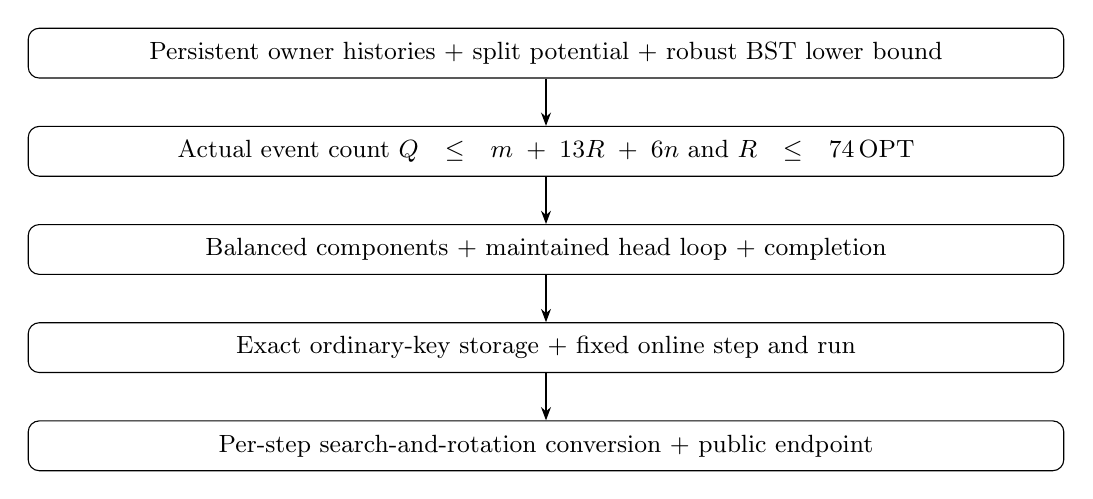
\begin{tikzpicture}[node distance=6mm, every node/.style={draw,rounded corners,
 align=center,font=\small,text width=128mm,inner sep=5pt},>=Stealth]
\node (a) {Persistent owner histories + split potential + robust BST lower bound};
\node[below=of a] (b) {Actual event count $Q\le m+13R+6n$ and $R\le74\OPT$};
\node[below=of b] (c) {Balanced components + maintained head loop + completion};
\node[below=of c] (d) {Exact ordinary-key storage + fixed online step and run};
\node[below=of d] (e) {Per-step search-and-rotation conversion + public endpoint};
\draw[->] (a)--(b); \draw[->] (b)--(c); \draw[->] (c)--(d); \draw[->] (d)--(e);
\end{tikzpicture}
\end{center}
The last box is the remaining assembly priority. Work on every stronger
machine model should stay off this path. In particular, bounded local
record discovery, prepared incoming cursors, cached header refresh,
constant-register code generation, and a persistent single-finger
simulation are not required by Definition~\ref{def:access}.

This is a change to the completion plan, not evidence that those earlier
lemmas were wrong. Many are checked and may support the stronger paper
implementation later. Preserve them and their proofs. The shared public
entry point should import the required mathematical route, while the
larger historical umbrella remains available for a full build and audit.
Deleting thousands of dependent source lines would create risk without
simplifying the theorem's assumptions.

The paper-to-Lean deviations are now explicit: weight-balanced instead
of red-black auxiliaries; root-first secondary repairs with the same
interval update; repaired first-visit accounting; a robust lower bound
valid for repeated keys; and an abstract online cost model instead of a
bounded local program. The first two change representation choices,
the next two repair mathematical arguments, and the last changes the
operational scope of the theorem. They should not be conflated.

Finish in this order: package the fixed natural-key transition; prove its
execution and prefix laws; derive the bound by the existing inequalities;
audit the common project; then decide whether the already available
linear initialization wrapper is worth exposing immediately. Do not
start arbitrary-universe padding or model-equivalence generalizations
before the minimal endpoint is reviewed.

\source{Short entry point: \lean{DynamicOptimalityResults.lean}.
The large historical entry point is \lean{ChaChaPaper20261030.lean}.
This guide supersedes older completion lists that made local controllers
mandatory for the current abstract target.}

\nextpage
\section{Classical MultiSplay: the exact algorithm matters}\label{sec:multisplay}
The requested next result concerns classical MultiSplay, not a newly
defined Cha-Cha variant that merely replaces its balanced
auxiliaries by splay trees. Classical MultiSplay uses a fixed node-storing
reference BST and represents its preferred paths by splay trees on the
original nodes. A splay operation moves its requested node to the root
by the standard zig, zig-zig, and zig-zag rotations.

For now use a perfect reference on $n=2^H-1$ keys, of height $H$.
Its external gaps provide $n+1$ ordered leaves for comparison with
leaf-oriented arguments, but these gaps are not additional keys. Every
preferred path has at most $H$ stored keys. The request visits wrong
proper ancestors in decreasing depth and then performs the mandatory
final switch at the requested node. This order differs from the
increasing-depth Cha-Cha head loop and must be transported explicitly.

The appropriate interface is a \emph{forest event word}: a chronological
list of root-splay searches, splits that splay and remove a specified
pivot, and raw root joins that put a specified pivot above two specified
components. Component identities and their ordered key domains are part
of the word. A raw join is not an arbitrary rebalancing operation.

For a left-to-right switch at $y$, let $U$ be the preferred prefix above
$y$, $L$ its old left tail, and $R$ the incoming right tail. Let $\ell$
and $r$ be the closest lower and upper ancestor keys of $y$ in $U$.
When both exist the prescribed word is
\begin{align*}
 &\operatorname{Split}(y),\quad\operatorname{Split}(\ell),\quad
   \operatorname{Split}(r),\\
 &\operatorname{Join}(A,\ell,\varnothing),\quad
   \operatorname{Join}(R,r,B),\quad\operatorname{Join}(A',y,B').
\end{align*}
Here $A,L$ are the daughters of the lower-guard split, and the upper-guard
split isolates $B$ from the empty gap beside $y$; $A',B'$ are the first
two joined results. The old tail $L$ remains as a parked component.
Missing guards omit their operations; right-to-left switching is reflected.

A comparator must execute this exact word on these domains. A cheap
Cha-Cha tree serving the same original requests is not
automatically such a comparator. This exact-word transport is the main
remaining mathematical step for MultiSplay.

\source{\lean{multisplay/common-forest-normal-form.tex};
\lean{multisplay/multisplay-competitiveness.tex}; the switch and replay
modules imported by \lean{MultiSplay.lean}. Original algorithm:
Wang--Derryberry--Sleator, \href{https://www.cs.cmu.edu/~jonderry/multi-splay.pdf}{SODA 2006}.}

\nextpage
\section{What the common-forest splay theorem already gives}\label{sec:forest}
Fix a forest event word $W$ as in Section~\ref{sec:multisplay}, and a
capacity $K$ bounding every live component's number of keys. A
\emph{comparator program} is an actual sequence of permitted operations
on these components, executing exactly $W$, with total budget $B$.
It may choose different internal shapes from splay, but it must respect
the same split pivots and join domains. A \emph{distinct splay trace}
is the supplied actual standard-splay execution of that word, with no
duplicated keys anywhere across the live forest.

The checked common-forest theorem states that there is a universal $C$
such that
\begin{equation}\label{eq:forest}
 \cost_{\rm splay}(W)\le
 C\bigl(N_0+r_0+B\bigr)g(K),
 \qquad g(K)=\operatorname{iteratedLog}(2,K)
             \operatorname{iteratedLog}(3,K)^2.
\end{equation}
Here $N_0$ is the sum of the sizes of the initial components, $r_0$ is
their number, and \lean{iteratedLog} applies the stabilized binary
ceiling logarithm repeatedly. The theorem assumes equal initial inorder
words, a capacity certificate, and the condition that each join fits
the capacity. Its conclusion concerns the supplied actual run, not
some alternative splay trace selected by the proof.

The difficult persistence issue has already been formalized: splitting
a component creates daughters whose histories inherit the parent's
state; joining components does not replenish their initial credit. The
proof passes through a persistent forest normalization and a packed
comparison, then transports the bound back using determinism of standard
splay. Empty components and permitted component permutations are handled
in the interface. There is one global initialization allowance, rather
than a new $O(K)$ charge for every short-lived component.

For classical MultiSplay, $K=H$, and the initial preferred-path forest
partitions $n$ keys, so $N_0=n$ and $r_0=O(n)$. What remains is to supply
the cheap comparator program for its exact forest word and to relate
the whole physical BST access cost to that replay. The theorem is not
conditional on an unproved splay competitiveness hypothesis; it reuses
the already checked shared splay analysis. Its \emph{input comparator}
is still a real obligation.

This is why the extension should reuse the common forest API instead of
rerunning the splay proof separately for each preferred-path lifetime.
The latter would lose the persistent accounting on which the desired
small factor depends.

\source{\lean{MultiSplay.CommonForest.forest_splay_bound} in
\lean{CommonForestSplayBound.lean}; \lean{DistinctSplayTrace.deterministic};
\lean{DistinctSplayTrace.toPointer}.}

\nextpage
\section{The MultiSplay extension: proved counters and the gap}\label{sec:msplan}
Let $S$ count actual classical MultiSplay switches, including final
switches, and let $F_{\rm act}$ count variation in the fixed-owner
secondary ledger of that exact chronological emission stream. For a
perfect node reference, Lean already proves
\begin{equation}\label{eq:ms-counter}
 m+S+F_{\rm act}\le2\,137\,120\OPT(X)+21n.
\end{equation}
This uses an endpoint-copy embedding, an arbitrary interval-hierarchy
lower bound, and a checked change-of-order argument. The primary state
may start arbitrarily; the secondary ledger is initialized rightward.
The theorem concerns the actual switches, not a sorted substitute word.

The hand draft \lean{chacha-common-forest-comparator.tex} proposes the
missing comparator. Its path component has genuine secondary interval
histories plus a structural boundary spine for the suffix beginning at
its top depth. A local depth request and splice should cost
$O((1+f)\lambda)$, where $f$ counts its genuine bit changes and
$\lambda=O(1+\log\log H)$. Structural boundary repairs must preserve
all deeper owner histories.

The proposed transport has three concrete obligations. First expose the
two external gaps adjacent to the switched key; their search paths
contain both existing ancestor guards. Second collect the touched
vertices into rooted skeletons, leaving identical untouched frontier
subtrees. Third reconfigure only these skeletons to insert the prescribed
three split and three raw join checkpoints. No rotation may cross a
current forest-component boundary. This must also work with empty tails
and missing guards. A generic same-key-set rotation theorem alone would
charge whole components and lose the required factor.

If this construction is proved, deleting omitted writes from each fixed
Boolean history cannot increase variation. It yields a comparator budget
$B=O(n+\lambda(S+F_{\rm act}))$. Combine with~\eqref{eq:ms-counter}
and~\eqref{eq:forest}, with $K=H$, and the global physical charging
described below, to obtain:
\[
 \cost_{\rm MS}(X)=O\bigl((\OPT(X)+n)\lambda g(H)\bigr)
 =O\bigl((\OPT(X)+n)(1+\log^{(3)}n)^2
                         (1+\log^{(4)}n)^2\bigr).
\]
Here $\log^{(j)}$ denotes $j$ repeated logarithms, stabilized at small
inputs. This is the proposed extension's factor; it is not the single
third-logarithm factor of Cha-Cha.

After the comparator, prove that the unchanged classical algorithm's
global search depth and rotations are charged to its actual switch
splays, including the final switch. Only then assemble competitiveness.
General-$n$ padding and any sharper black-box splay factor come later.

\source{\lean{MultiSplay.EndpointEncoding.perfect_reference_actual_counters_le_OPT};
\lean{multisplay/composition-audit.tex};
\lean{multisplay/chacha-common-forest-comparator.tex}. The latter remains
a hand proof to formalize and audit.}

\nextpage
\section{Completion criteria and an audit trail}\label{sec:verification}
The first deliverable is a public theorem for a fixed online
Cha-Cha strategy on the agreed power-of-two universe,
with its actual initial tree and the search-and-rotation bound in
Section~\ref{sec:constants}. It must expose enough of the strategy to
check that every step serves its requested key and transforms the same
tree used by the next step. A theorem with a user-supplied cheap simulator
or a missing representation invariant is not this deliverable.

The endpoint should export four connected facts: the inorder word of
every boundary tree is exactly the original key range; the selected
steps form an actual \lean{SearchRotation.Execution}; appending requests
preserves the already chosen prefix state and cost; and that cost obeys
the shared-OPT bound. The competitor corollary then follows from
\lean{SearchRotation.OPT_le_cost}. If arbitrary initial trees are exposed,
their initialization is performed and charged once, with an empty word
leaving the supplied initial tree unchanged.

At the project root the reproducible commands are
\begin{verbatim}
make lean
make audit
make guide
\end{verbatim}
The Lean build uses the common dependency cache and serializes builds
through the workspace lock. The audit collects axiom dependencies of
public and private declarations in the shared, splay, Greedy, Cha-Cha, and
MultiSplay namespaces. It accepts only the standard logical axioms
\lean{propext}, \lean{Classical.choice}, and \lean{Quot.sound}.
No \lean{sorry}, new assumption, or unchecked native proof is permitted.
An axiom audit validates proof dependencies; reviewing theorem hypotheses
and definitions remains necessary to validate the mathematical scope.

The authoritative source locations for this guide are the preserved
30 October paper under \lean{chacha/imports/2026-10-30-ChaCha/paper/},
the corresponding Lean namespace \lean{ChaCha.Paper20261030},
the shared \lean{DynamicOptimality/} directory, and the existing
\lean{multisplay/} drafts and formalization. Corrections to the imported
paper are recorded in \lean{PROOF_REPAIRS_2026_10_30.md}; the original
archive is not silently edited to match the formalization.

At the preparation of this document, the lower bound and fixed-strategy
metadata cost theorem are complete; the natural-key abstract endpoint
is the next assembly task. Classical MultiSplay has a checked persistent
forest comparison and actual counter theorem, but the exact-word physical
comparator and final BST assembly remain. Local-controller implementation,
arbitrary-universe padding, and broader machine-model comparisons are
explicitly deferred. Subsequent endpoint changes should be recorded in
a short dated verification note rather than retroactively treating this
planning snapshot as if it had already contained them.
\nextpage
\section{Completion: removing the universe-size restriction}\label{sec:padding}
After the initial twenty-page proof review, the abstract endpoint was
completed and then extended to every finite universe. This section records
the additional argument. Write $\pi_n(T)$ for \emph{prefix pruning}: retain
the keys smaller than $n$ in an ordered tree $T$. Recursively, a retained
root keeps its two pruned children; a root at least $n$ is replaced by
its pruned left subtree. Its entire right subtree is too large to survive.

One ordinary rotation projects to zero or one ordinary rotations. If both
rotated keys survive, perform the same rotation. If exactly one survives,
the two pruned shapes coincide; if neither survives, they also coincide.
The impossible ordering of a retained larger key above a deleted smaller
key is excluded by BST order. Context rotations lift recursively. Also,
a search for a retained key follows its old route with some vertices
removed. Thus an entire access projects to an access with the exact
pruned endpoints and no larger initial search depth or rotation count.

For arbitrary $n>0$, choose $h=\clog n$ and $N=2^{h+1}$, so
$n\le N\le4n$. Run the completed strategy on this virtual universe, but
make its \emph{actual} BST $\pi_n(T)$. Its internal state retains the
virtual state as free bookkeeping. Fix each projected transition using
only that state and the current original request. The shared online
interface then supplies actual executions and exact prefix consistency.
No virtual key appears in the physical BST.

Extend a supplied initial $n$-key tree by placing it below a new root
$n$ with the remaining larger keys on the right. Pruning recovers the
\emph{exact} supplied tree. The same extension of any competitor adds
one to each original search depth and leaves its rotation count unchanged.
The two shared root-service conversions from Section~\ref{sec:opt} give
$\OPT_N(X)\le6\OPT_n(X)$. With $C=134\,880\,000\,019$, the completed
power-of-two bound therefore yields
\[
 \cost_n(X)\le6C(\OPT_n(X)+n)L(\clog n).
\]
Finally, write $\ell_j(n)$ for the shared stabilized $j$-fold logarithm.
The checked numerical bound $L(\clog n)\le4\ell_3(n)$ gives the public
theorem \lean{DynamicOptimality.ChaCha.All.third_log_competitive}:
\[
 \cost_n(X)\le3\,237\,120\,000\,456(\OPT(X)+n)\ell_3(n).
\]
It uses the unrestricted shared \lean{Competitive} definition, every
initial BST, and the actual search-and-rotation cost. The empty universe
has only the empty request word and costs zero. Only the stronger local
machine implementation and the classical MultiSplay extension remain
outside this completed theorem.

\source{\lean{SearchRotationProjection.lean}; \lean{OnlineBSTProjection.lean};
\lean{UniverseExtension.lean}; \lean{PaddingSize.lean};
\lean{PaddingFactor.lean}; root \lean{ChaChaAll.lean}.}
\end{document}
